%%%%%%%%% PROJECT DESCRIPTION  -- 15 pages (including Prior NSF Support)

\required{Project Description}
%\begin{center}
%\emph{Maximum of 6 pages}
%\end{center}
%The Project Description (including Results from Prior NSF Support, which is limited to five pages) may not exceed 15 pages. Visual materials, including charts, graphs, maps, photographs and other pictorial presentations are included in the 15-page limitation. PIs be cautioned that the project description must be self-contained and that URLs that provide information related to the proposal should not be used. 

%All proposals to NSF are reviewed utilizing the two merit review criteria, intellectual merit and broader impacts. 

% The Project Description should provide a clear statement of the work to be undertaken and must include: objectives for the period of the proposed  work and expected significance; relation to longer-term goals of the PI's project; and relation to the present state of knowledge in the field, to work in progress by the PI under other support and to work in progress elsewhere.

%%%%%%%%%%%%%%%%%%%%%%%%%%%%%%%%%%%%%%%%%%%%%%%%%%%%%%%%%%%%%%%%%%%%%%
%INTRO
% a brief and informative introduction or background section
%%%%%%%%%%%%%%%%%%%%%%%%%%%%%%%%%%%%%%%%%%%%%%%%%%%%%%%%%%%%%%%%%%%%%

\vspace{-0.6cm}
\section*{A. Introduction} \vspace{-1ex} % should not repeat the summary page

A critical goal of evolutionary biology today is to understand organisms' abilities to adapt to new or changing conditions. This is especially relevant in the face of global climate change and other increasingly common anthropogenic changes to the environment \citep{Easterling:2000ja}. Most ecologically or economically important phenotypic traits have a complex, quantitative genetic basis, and considerable heterogeneity exists within and among species in this genetic architecture---the number of causal loci, their effect sizes, and allele frequencies \citep{orr:2001, slate:2005}. Yet we know very little about how the genetic architecture shapes, and is shaped by, the process of adaptation. In order to understand the maintenance of variation or adaptive potential of phenotypes of interest, we must understand how their genetic architecture changes as a result of evolutionary processes such as selection and demography, and how differences in genetic architecture may limit adaptive change. Such knowledge advances our understanding of the process of adaptation and can further benefit crucial goals such as improving crop yields under changing climates. 

Nearly all knowledge of adaptation comes from population genetic theory focusing on single loci or quantitative genetics theory that evaluates variances and ignores the underlying loci. Yet theoretical analysis of simple models of quantitative traits have shown that neither of these approaches can successfully predict the impact of evolutionary processes on the genetic diversity of loci underlying quantitative traits \citep{Chevin:2008, LeCorre:2012co}. 
While quantitative trait locus (QTL) mapping approaches and genome-wide association studies (GWAS) have successfully identified a number of causative loci, these methods suffer from statistical issues limiting their utility for studying genetic architecture of adaptive traits \citep{spencer2009designing,Gibson:2012,Thornton:2013}. Alleles missed in most QTL or GWAS studies may nonetheless be of central importance to adaption \citep{Rockman:2011ej, Mackay:2009}, and novel approaches are thus needed to understand how evolutionary processes affect the architecture of quantitative traits.

The genetic architecture of a trait is determined by a number of factors, including population size, mutation, demographic history, and the history of both purifying and positive selection. Population bottlenecks, for example, can lead to the loss of variation or maintenance of deleterious variation \citep[e.g.][]{Renaut:2015hi, Gunther:2010}. Strong selection, such as that imposed during crop domestication, can fix large-effect loci \citep{Brown:2011}. Both theoretical and empirical studies in humans have shown that the genetic architecture of human traits is shaped by the frequency and effect size of mutations \citep{Thornton:2013} as well as the interaction of demographic and selective histories \citep{Fu:2014jt, Gravel:2011iq, Henn:2015dp}.

This proposal aims to develop a simulation framework that allows explicit modeling of the evolution of the genetic architecture of a quantitative trait. This model will then be used to investigate how different factors shape the architecture of quantitative traits in maize and its wild relative teosinte. Thanks to its economic importance and history as a model genetic organism, extensive genomic \citep{Wright:2005,Hufford:2012dy} and phenotypic \citep{Wallace:2014,Weber:2009} data exist for both maize and teosinte, making it an ideal system in which to study processes affecting genetic architecture.  

\textbf{I propose four objectives which make use of the extensive knowledge and data available in the maize\//teosinte system in order to develop an explicit genomic model of the evolution of a quantitative trait.} Objective \ref{modeling} builds a simulation model fit to empirical estimates of the genetic architecture of phenotypically important traits in the wild ancestor of maize. Objective \ref{domestication} then uses simulations of maize domestication and comparisons to empirical data to understand how demography and selection combined affect the genetic architecture of phenotypes in maize.  Objective \ref{validation} empirically tests  predictions made in Objectives \ref{modeling} and \ref{domestication} by comparing the effects of maize and teosinte alleles in a common genetic background in two mapping populations. Finally, Objective \ref{surfing} uses our simulation model to predict changing genetic architecture in maize landraces as they spread across the Americas post-domestication and how variable their adaptability may be into the future. This research has tremendous opportunity to further our understanding of the impact demography and selection have on phenotypic traits and their underlying genetics. Such knowledge greatly improves our ability to predict the effects of selection and changing environments on the genome as well as to exploit genetic diversity in crops for continued breeding or any species of concern for future conservation. \vspace{-3ex}

%%%%%%%%%%%%%%%%%%%%%%%%%%%%%%%%%%%%%%%%%%%%%%%%%%%%%%%%%%%%%%%%%%%%%%
%OBJECTIVES
% a statement of research objectives, methods, and significance
%%%%%%%%%%%%%%%%%%%%%%%%%%%%%%%%%%%%%%%%%%%%%%%%%%%%%%%%%%%%%%%%%%%%%%

\section*{B. Research Objectives, Methods \& Significance}\vspace{-1ex}

\renewcommand\thesubsection{\Roman {subsection}.}

\subsection{Model the genetic architecture of phenotypes in teosinte}\vspace{-1ex}
\label{modeling}
In Objective \ref{modeling} I will build a model to simulate the genetic architecture of phenotypes in the wild ancestor of maize, teosinte (\emph{Zea mays} ssp. \emph{parviglumis}). This model will then enable us to study the impacts of demography and selection on the genetic basis of phenotypic traits during domestication (Objective \ref{domestication}) and range expansion (Objective \ref{surfing}).

In order to model the architecture of quantitative traits, I first need to understand the effects of mutation. The distribution of fitness effects (DFE) describes the consequences of mutations in terms of their impacts on an organism's fitness. Taking advantage of published \citep{Chia:2012} and ongoing whole-genome sequencing data in teosinte (see Data Management Plan), I will estimate the DFE in teosinte with the software DoFE \citep{Keightley:2007hq, Stoletzki:2011}. The resulting estimates of the fitness effects of new mutations can then be parameterized in terms of their effect on fitness-related quantitative traits \citep{Keightley:1988, eyre-walker:2010}, including yield, plant height, and flowering time.

This estimated DFE, combined with prior information on mutation \citep{Clark:2005} and recombination rates \citep{Rodgers-Melnick:2014}, will then be used as input in simulation models of quantitative trait evolution in teosinte. Additional parameters necessary for our model (including dominance and the correlation between a trait and fitness) will be estimated using an Approximate Bayesian computation (ABC) approach \citep{Beaumont:2002ue}. I will draw simulation parameters from a prior distribution and then compare summary statistics generated by simulation to observed data. By keeping the parameter draws that generate data most similar to the observed data, I can estimate the parameters' posterior distributions. I will take advantage of the library fwdpy (a Python implementation of fwdpp \citealt{Thornton:2014kn}, available at \url{https://github.com/molpopgen/fwdpy}) to write simulation code that explicitly models a quantitative trait evolving under a model of stabilizing selection. From each simulation, I will then perform genome-wide-association analysis in order to compare model results with observed data from published \citep{Weber:2009} and on-going (see Data Management Plan) analysis of 16 phenotypic traits in a natural population of teosinte. ABC will allow robust estimation of the necessary parameters from a set of several million such simulations.

\vspace{-2ex}
\paragraph{Significance}
Good estimates of the DFE are currently available for very few plants, and very few species in general, but inform models of both population and quantitative genetics, including for example the genetic basis of heterosis \citep{Mezmouk:2014jd} or the genetic basis of complex diseases \citep{EyreWalker:2007dl}. Estimates of the DFE also contribute to future studies aiming to realistically simulate any distribution of mutation effects by further describing the variability of this distribution across species. Most importantly, this objective will produce a functioning model of selection on quantitative traits, allowing for the first time simulation of how evolutionary processes impact diversity at the genes underlying quantitative traits. 

\vspace{-1ex}	
\subsection{Model quantitative genetics of maize domestication}\vspace{-1ex}
\label{domestication}
The model developed in Objective \ref{modeling} will enable simulation of quantitative traits under stabilizing selection. Here I will build upon this model to incorporate both demographic change and directional selection in order to investigate the impact of domestication on the genetic architecture of phenotypes of interest. Both demographic change associated with a domestication bottleneck and directional selection are expected to change the architecture of quantitative traits, but a detailed understanding of how these two forces interact is lacking. I predict that traits under directional selection will be enriched for large effect alleles, as these contribute to greater phenotypic change, while traits under stabilizing selection are expected to have a deficit of large effect alleles as these are selected against to maintain the optimal phenotype (e.g. Figure \ref{fig:model}).

To test this prediction, I will extend the simulation framework developed in Objective \ref{modeling} to include estimates of population size change during the domestication bottleneck and subsequent expansion \citep{Wright:2005}. Using the parameters estimated for teosinte, I will simulate the same quantitative traits in a population undergoing a domestication bottleneck. This first analysis provides a null expectation of the genetic architecture of traits in the absence of directional selection. Differences between simulated and observed data \citep[][and our own on-going analyses---see Data Management Plan]{Wallace:2014} are informative for the history of selection on phenotypes. I will again use an ABC approach and GWAS of simulations performed using fwdpy to estimate the strength of selection on domestication phenotypes and re-simulate with more accurate selection parameters to assess how traits experiencing varying strengths of selection and with varying heritability have changed over the course of domestication.

Traits believed to evolve neutrally during domestication may only be impacted by demographic forces of the domestication bottleneck, while other traits are thought to have simultaneously experienced directional selection. Traits with high heritability or traits under stronger directional selection may change more dramatically than those evolving neutrally while subject to the bottleneck. I can thus test if allelic effect sizes have shifted their distribution mean or overall shape to more or fewer loci of large effect \citep{Chevin:2008} depending on the strength of selection. 
Traits in maize such as kernel weight and kernel row number, among other ear-related traits (Figure 1), are expected to have been selected for crop improvement, while there are no strong reasons to suspect other traits such as total plant height were under selection. This suite of traits thus provides us with \emph{a priori} predictions on which traits should show differences from our simple demographic simulations, and cases where these predictions are not matched may indicate genetic correlations with selected traits that could be confirmed by reanalysis of data from published GWA studies. 

%\vspace{-0.4cm}
\begin{SCfigure}[][t]
\vspace{-2ex}
\centering
   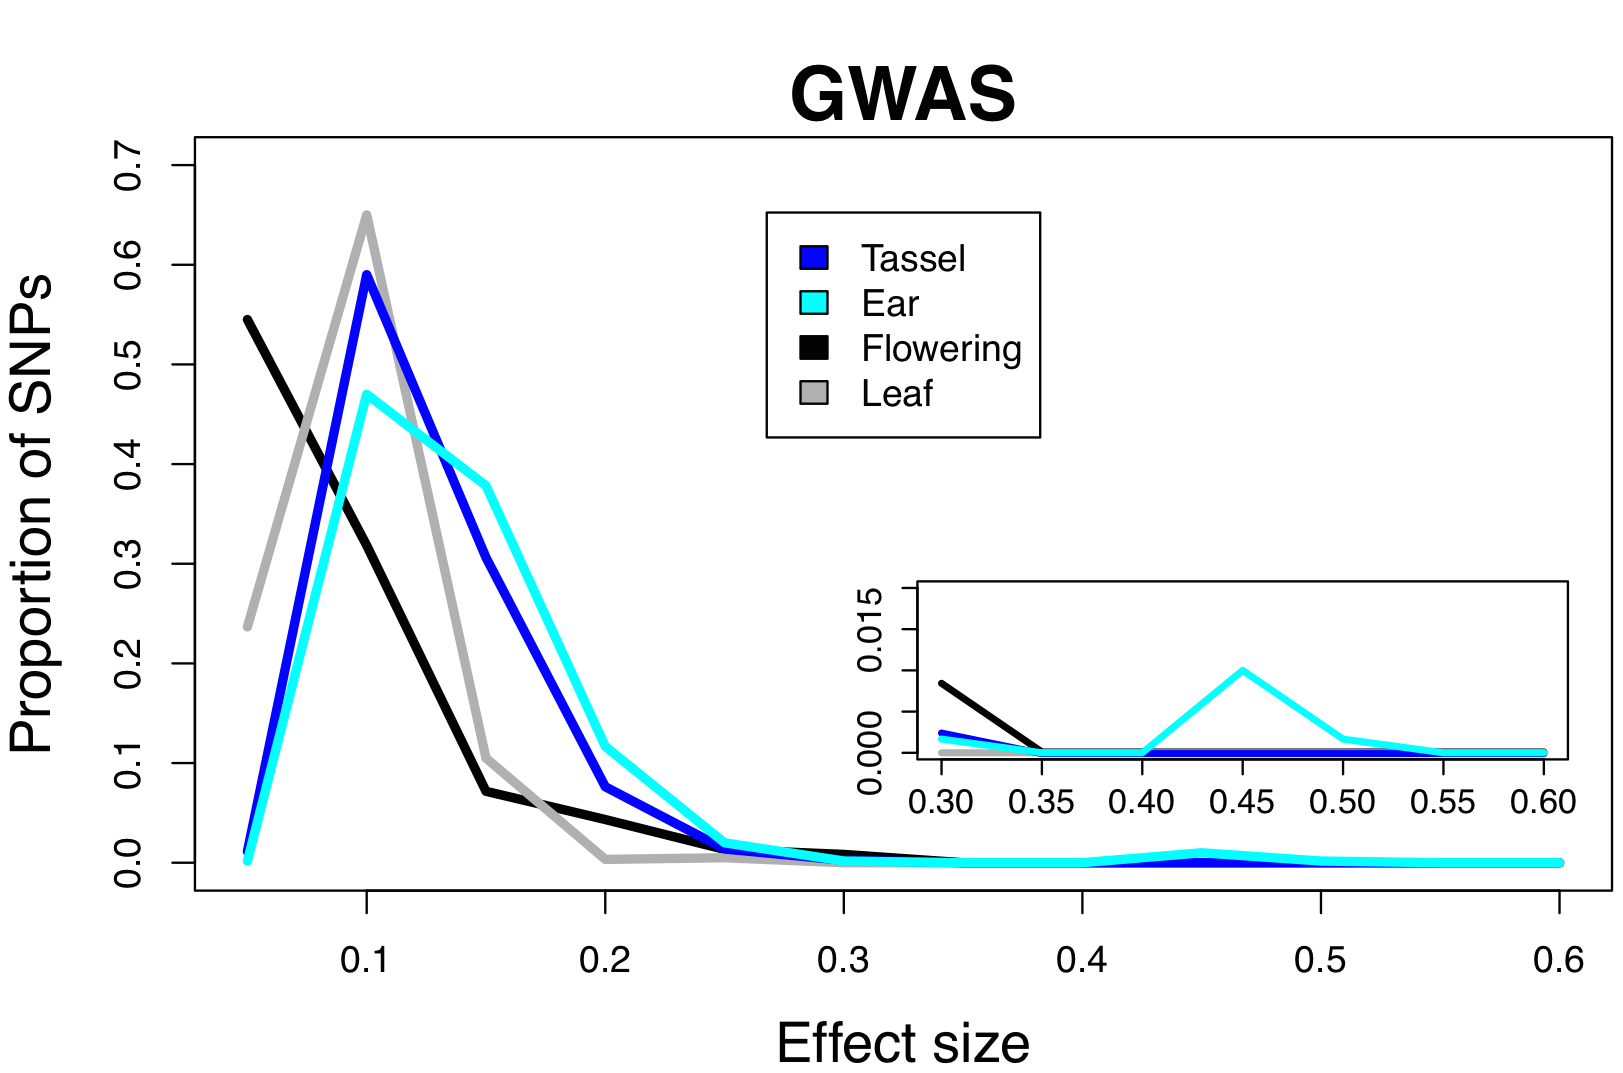
\includegraphics[width=0.55\textwidth]{Figure2_Brownetal2011.png}
  \caption{Effect sizes from GWAS analyses in maize, grouped by trait category. Inset shows the largest effects. Ear traits, showing the largest effect sizes, were likely selected during maize domestication while the others were not. Figure from \citealt{Brown:2011}.}
  \label{fig:model}
\vspace{-2ex}
\end{SCfigure}
	
\vspace{-2ex}
\paragraph{Significance}
The results of this Objective will allow us to distinguish the relative importance of demography and selection in determining the genetic architecture of maize. 
The impact of demography on the genetic architecture of traits is not well understood in any system. How population bottlenecks affect deleterious variants of different effect size remains controversial in humans, for example \citep{Hancock:2011jb, Henn:2015ce, Henn:2015dp, Lohmueller:2014dn, Simons:2014fj}. The effects of these processes vary depending on the degree of population size reduction and the length of time over which populations are bottlenecked \citep[e.g.][]{Caplins:2014ke}, but also have the potential to interact with selection. In crops, for example, it has been argued that smaller population sizes and selection together have lead to an increase in the frequency of deleterious alleles  \citep{Gunther:2010, Renaut:2015hi}. Consistent with this, it has recently been shown that genes associated with a number of quantitative traits in maize are enriched for deleterious alleles compared to randomly chosen genes \citep{Mezmouk:2014jd}. Understanding this information is crucial for understanding variation in phenotype, designing breeding strategies, utilizing diversity from wild relatives, or even engineering new traits using biotechnology. 

\vspace{-1ex}
\subsection{Validate model predictions in synthetic mapping populations}\vspace{-1ex}
\label{validation}

Models developed in Objective \ref{modeling} and \ref{domestication} lead to direct predictions of the genetic architecture of quantitative traits and how they should differ between maize and teosinte. To validate the predictions of these models, I will take advantage of two mapping populations containing mixtures of teosinte and maize alleles: a set of near isogenic lines of teosinte alleles introgressed into a maize background \citep{Liu:InPress}, and a synthetic population resulting from the cross of 11 teosinte and 26 maize parents (see Data Management Plan). Genotype and phenotype data are available for both populations, and if necessary I will add additional genotyping to augment marker density. I hypothesize that teosinte will have a wide range of effect sizes across loci, while in maize, domestication traits should have more large effect alleles than teosinte, and neutral traits more small effect loci due to purging of detrimental large effect alleles during domestication. I will perform a GWAS on these samples for the traits already used to calibrate our models. Identification of GWAS hits in regions of the genome coming from maize and teosinte will allow us to compare the effect size distribution of causal variants in a common environment and genetic background. With information on the correlation between phenotype and fitness, our model and simulations should be able to predict the difference in genetic architecture for new traits. I will thus perform a similar analysis for traits not included in our calibration to test the predictive ability of our model. 

\vspace{-2ex}
\paragraph{Significance}
Objective \ref{modeling} and \ref{domestication} allow us to understand differences in genetic architecture based on fitting simulations to empirical data. This objective will demonstrate the predictive ability of our model for new phenotypes in a mapping population not used for model development; thus directly testing its potential utility in other systems.

\vspace{-1ex}
\subsection{Investigate the impact of demography and local adaptation of maize landraces across the Americas} \vspace{-1ex}
\label{surfing}

After domestication, maize spread across Central and South America, adapting to a variety of environments across a wide elevational range. These populations have experienced further demographic and selective pressures in addition to an initial domestication bottleneck. For example, South American populations are inferred to have experienced a second severe bottleneck \citep{Takuno:2015eu}, and more generally populations expanding geographically are likely to have experienced serial founder effects that can change allele frequencies in unexpected ways due to allele surfing \citep{Klopfstein:2005bl}. The effect of range expansion on deleterious alleles remains controversial \citep{Henn:2015ce, Henn:2015dp, Simons:2014fj, Sudmant:2015}, and even less is known about its impact on quantitative traits. Changing selection pressures from both new environments and artificial selection by different human populations likely also interact with these demographies. 

%Demographic bottlenecks are common during the geographic spread of populations and can have several effects on the genome including purging of deleterious alleles (recessive alleles become homozygous and are more efficiently removed), or alternatively may lead to an increase of some deleterious alleles through increased random genetic drift (allele surfing, \citealt{Klopfstein:2005bl}).

In this objective, I will simulate quantitative traits for populations undergoing multiple shifts in selection as well as additional demographic change to incorporate range expansion and further bottlenecks. I hypothesize that the genetic architectures with more large effect alleles that are deleterious and fewer that are beneficial might evolve. \kjg{from increased genetic drift during periods of reduced population size during bottlenecks and expansion - make sense?}
%deleterious alleles\kjg{predictions from allele surfing} as well as a loss of potentially beneficial alleles of large effect. 
I will compare these predictions to GWAS results from publicly available genotype and phenotype data of nearly 5,000 landraces from across the Americas \citep{Hearne2015}. Furthermore, I hypothesize that these changes in genetic architecture may limit future adaptive ability of populations. To test this, I will impose identical shifts in selection on each resulting architecture and assess each population's response in terms of speed and magnitude of phenotypic change. It is hypothesized that architectures containing more loci of small effect have genetic redundancy that benefit adaptation to new conditions.

\vspace{-2ex}
\paragraph{Significance}
This allows assessment of how complex demography and changing selection regimes affect the genetic architecture of local adaptation to different conditions. It will also further test predictions on how future adaptation may be impacted by current genetic architecture \citep{Yeaman:2015cc}. Understanding the characteristics that lead to this improved ability to adapt allow more predictability of evolutionary processes and better methods of artificial selection or conservation efforts to ensure the persistence of crops and other species of importance for biodiversity into the future.
\vspace{-3ex}

% latex FTW :)

%DELETED Maize originated approximately 9,000 years ago in southern Mexico (cite Matsuoka et al 2002, others?) during a single domestication event of \emph{ssp. parviglumis}. Archaeological records also confirm this dating and single location (cite) as well as the subsequent spread and growth in population size of domestic landraces across the Americas into both lowland and highland environments [cite Wilkes, H. G. (1967) Teosinte: The Closest Relative of Maize (Harvard Univ., Cambridge, MA)]. South American landraces of maize also underwent a second bottleneck event during their expansion (cite). Using genetic data, the precise demographic parameters of this history have been estimated (cite Beissinger et al in prep). This provides information on the ancestral effective population size of maize ($N_a \approx$ 120,000), the size to which the population was bottlenecked during domestication (5\% of this $N_a$), the subsequent size to which populations rapidly expanded (3 times as large as $N_a$\kjg{but maybe as much as 1E9, citation}), and lastly on the genome-wide mutation rate ($3.8\times10^-8$ cite Clark et al 2005 MBE 22, 2304 -- 2312.)

%DELETE? These individuals will occupy populations that will be subjected to combinations of demographic and selective pressures including some of the following. To recapitulate the various landraces of maize, I will include cases of a second bottleneck after the domestication bottleneck, populations undergoing little or significant additional range expansion (Central American versus South American), stronger or weaker selection on flowering time and phenological traits (warmer lowland versus colder highland adapted populations), and cases with or without gene flow from sympatric\kjg{is that accurate, there is teosinte around them at least?} populations of teosinte.
%\jri{ambivalent about the teosinte idea. on one hand very cool and lots of additional questions -- adaptive introgression, maladaptive gene flow, etc. on the other hand, further complication and another layer to add to already complex grant. inclined to skip for space reasons.} -agreed-kjg

%DELETED: The objective of this project is to simulate the impact of multiple demographic events and selective pressures either individually or in combination. This will show how much variation is possible in terms of the effects on genetic architecture underlying traits for adaptation. The core set of simulations in this project will be designed to match the known landraces in maize, but will include more broadly a designed experiment to compare the presence or absence of particular evolutionary forces. Using genomic and phenotypic data for some landrace populations of maize (see Data below), I can compare a subset of these simulations to real data to assess how well these simulation results match real populations across the species range. The goal of this project is to inform our understanding of the relative importance or insignificance of the tested demographic cases and how sensitive genetic architecture is to these.

%\subsection*{Data}
%This project will make use of both published data as well as data generated or currently being generated as part of a related Plant Genome project (Biology of Rare Alleles IOS-1238014) of which sponsoring scientist Dr. Ross-Ibarra is a Co-PI. As part of this project, Dr. Ross-Ibarra's group is currently in the process of sequencing 70 teosinte and 55 maize genomes to high depth. These sequences should be complete by the end of 2015 and will be made publicly available early 2016 via the group website (\url{www.panzea.org}). The individuals used for genome sequencing are also the parents of two large mapping populations of $\sim$5000 progeny. Both populations have been genotyped and phenotyped for a number of traits including seed yield, flowering times, and plant height, and would be used for comparisons in Objectives \ref{modeling} and \ref{domestication}. Finally, the same project has developed, genotyped, and phenotyped a  synthetic population of 11 teosinte and 26 maize parents, resulting in a population that is roughly 12\% teosinte genes, 40\% B73 (the reference genome line), and 2\% from 25 other inbred maize lines. This latter population will be used in Objective \ref{validation} to compare model predictions to maize and teosinte regions segregating in a common population.  All of these data are currently available from collaborators.  Publication of results from analyses of these data must await publication of collaborators' GWAS analyses, but as these are currently underway and comparisons with empirical data would likely not begin until early 2017 at the soonest we do not foresee this being an issue. In the unlikely event of a problem in the generation of that data, existing data is also available publicly for teosinte \citep{Weber:2009} and maize \citep{Wallace:2014} as well as $\sim$1500 maize genomes through the HapMap 3 project \citep{Bukowski:2015} and 4,000 landraces each with 1 million SNPs and several phenotypes \citep{Hearne2015}.


% NB if you prefer \approx, let me know! I've just been changing them to \sim because in my head I read that as "approximately" whereas I read the former as "approximately equal to", but that may just be me

%_________________% DATA INFORMATION %_________________%

%%%RARE ALLELES PROJECT (probably the most useful data)
% 1 pop of teo w/ 70 parents (sequenced), 5000 progeny (16 phenotypes, GBS, imputation in progress)
% 1 pop of landrace maize w/ 55 parents (sequencing in progress), 5000 progeny (~25 (?) phenotypes, GBS, imputation in progress)
% 4 additional teo pops,  each with 10 parents (sequencing in progress) and 1200 progeny (GBS done, phenotyping in progress done in Jan 2017)
% 4 additional landrace maize pops,  each with 10 parents (sequencing in progress) and 1200 progeny (GBS done, phenotyping in progress done in Jan 2017)

%%OTHER DATA OF USE
% for teosinte architecture
% Weber 2009 teosinte population (if DNAs still available; may be too small sample size pop) 

%for architecture of traits in maize

% NAM!! 5000 RILs, GBS, 42 phenotypes    26 parents crossed to an additional line, 15 million snps


%(suboptimal) alternative DFE, diversity data
% ~1500 sequnced maize genomes (Hapmap 3 and 4) 

%for comparison of maize and teo architecture
% teosinte synthetic: ~2500 DH lines, ~12% teosinte, 40% B73, 2% of each other 25 NAM parents there is dna and tissue
% Briggs 2007 mapping population (600 BC2S3 to estimate ), maybe genotyped on ~1500 markers
% Sherry parviglumis NILs (~800??) there are seeds

% for looking at other landraces
% ~6 landrace genomes each from highland mexico, lowland mexico, highland S. america, lowland s. america, highland guatemala, US southwest
% SeeDs: 
	% 4,000 landraces each w/ 1M SNPs and several phenos (publicly available)
	% 25,000 landraces, each w/ pooled seq. of ~30 plants. + some phenos (not yet avaible, but we know the woman in charge of the program)
	
% other goodies
% 0.2cM-scale recombination map
% rho-map (starting Feb. 2016)
%___________________________________________________%	

	
%%%%%%%%%%%%%%%%%%%%%%%%%%%%%%%%%%%%%%%%%%%%%%%%%%%%%%%%%%%%%%%%%%%%%%
%TRAINING OBJECTIVES
% training objectives and plan for achieving them (these may include scientific as well as other career preparation activities)
%%%%%%%%%%%%%%%%%%%%%%%%%%%%%%%%%%%%%%%%%%%%%%%%%%%%%%%%%%%%%%%%%%%%%%
\section*{C. Training Objectives}\vspace{-1ex}
This fellowship will provide me with an ideal opportunity to learn the skills needed to enhance my ability to conduct cutting edge research in the fields of genomics and computational biology, both areas in which I expect to continue my future research and which are greatly expanding in evolutionary biology. I will gain many skills related to genomic data analysis through these projects, learning bioinformatics and analysis skills for large datasets. I have limited experience working with genomic data from my dissertation, thus making this a vital step in my career. Genomic technology and data are growing at an incredibly fast pace, and working directly with such data will teach me the most up to date, accurate, and efficient approaches. I will also improve my computational biology skills through the proposed simulations, learning a new and useful programming language, Python, that I can apply throughout this research and my future research in evolutionary biology. \vspace{-3ex}

%%%%%%%%%%%%%%%%%%%%%%%%%%%%%%%%%%%%%%%%%%%%%%%%%%%%%%%%%%%%%%%%%%%%%%
%CAREER DEVELOPMENT
% an explanation of how the fellowship activities will enhance your career development and future research directions as well as describing how this research differs from your dissertation research, thus providing you an opportunity to broaden your scientific horizon
%%%%%%%%%%%%%%%%%%%%%%%%%%%%%%%%%%%%%%%%%%%%%%%%%%%%%%%%%%%%%%%%%%%%%%
\section*{D. Career Development \& Future Research}\vspace{-1ex}
My career goal is to develop an innovative research program in evolutionary biology, studying population genetics and processes that impact genetic diversity. I believe such research is key for the future, not only for the field of evolutionary biology, but also in applied scenarios such as understanding prevalence of genetic diseases in humans, adaptation of species to climate change, or strategies to improve agricultural products for a growing world population. My dissertation research has approached some of these questions in a more theoretical and less applied mindset. The work I will conduct during this fellowship would have more direct potential for application in the field of maize agriculture. For me, this is necessary and vital experience for my career development as I decide between pursuing a more applied research program, potentially in industry or government research scientist positions, or in pursing a career as an academic researcher at a university.

The skills I will develop during this fellowship, as described in section C, will benefit my career and put me on the cutting edge for analyses of the newest genomic data and the most recent computational approaches for biological simulations. Interacting with Dr. Ross\--Ibarra, as well as other researchers at UC Davis, and with Dr. Kevin Thornton at UC Irvine, will be both intellectually stimulating and rewarding experiences that will help me accomplish my career goals. Drs. Ross\--Ibarra and Thornton are both at the forefront of a popular movement for open science, making all stages of the research process transparent to any interested parties, and providing products such as data and code immediately and publicly. This is a work ethic I strongly agree with and hope to contribute to as an independent researcher. Our work together will better equip me with the tools and experience that make open science efficient, and rewarding for all. I believe that this will equip me as a competitive, knowledgeable, and independent researcher able to conduct interesting and useful research throughout my future research program on topics of local adaptation, demographic history, population structure and genetic architecture of important traits. Furthermore, Dr. Ross-Ibarra has an excellent track record of helping his post-doctoral fellows secure promising positions for their future careers, including three assistant professorships at universities, 3 research scientist positions in the seed industry, one at an NGO, and one in the USDA.\vspace{-3ex}

%%%%%%%%%%%%%%%%%%%%%%%%%%%%%%%%%%%%%%%%%%%%%%%%%%%%%%%%%%%%%%%%%%%%%%
% HOST INSTITUTION
% a justification of the choice of sponsoring scientist(s) and host institution(s)
%%%%%%%%%%%%%%%%%%%%%%%%%%%%%%%%%%%%%%%%%%%%%%%%%%%%%%%%%%%%%%%%%%%%%%
\section*{E. Sponsoring Scientists and Host Institution}\vspace{-1ex}

The University of California Davis (UCD) is the ideal place to conduct the proposed research. UCD has a world-renowned program in evolutionary biology and faculty in population genetics who are leaders in the field. Jeff Ross\--Ibarra is an expert on teosinte, maize, its domestication, and the associated population genetics and genomics of the system. Kevin Thornton is an accomplished quantitative geneticist and computational biologist at UC Irvine, who will contribute greatly to this research. Both will serve as effective and capable mentors for my post-doctoral research. In particular, Jeff has been studying the maize\//teosinte system for years with a great network of collaborators providing vast resources of data. His work has contributed largely to our knowledge of this system, and more generally on domestication and adaptation as evolutionary processes. Kevin is the developer and maintainer of fwdpy, the python package proposed for completing the simulations. He will thus serve as a great resource in terms of knowing the exact capabilities of the simulation method and assumptions of its model that must be taken into account. Furthermore, the Department of Ecology and Evolution, the Department of Plant Biology, and the Department of Plant Sciences at UCD have many exceptional faculty doing research relevant to my interests, providing many research groups to interact with on a daily basis for potential collaborations or feedback on this research. I look forward to interacting with scientists interested in population genetics, such as Graham Coop, and in adaptation, such as Johanna Schmitt. %Additionally, experts in plant regulatory evolution, such as Neelima Sinha, Siobhan Brady, and Daniel Runcie will serve as great people to interact with. % need to look up people in the dept, these names were just taken from Emily J's application
UCD and UC Irvine both have extensive computing resources for our proposed work with access to dedicated processors and nodes across multiple clusters of large RAM capabilities (see Sponsoring Scientist Statement), and as described, vast sources of knowledge and experience on the topics I plan to investigate, ensuring the success of this work. I am excited to join and contribute to such an active and vibrant scientific community.\vspace{-3ex}

%%%%%%%%%%%%%%%%%%%%%%%%%%%%%%%%%%%%%%%%%%%%%%%%%%%%%%%%%%%%%%%%%%%%%%
%Milestones
% a timetable with yearly goals with benchmarks for major anticipated outcomes
%%%%%%%%%%%%%%%%%%%%%%%%%%%%%%%%%%%%%%%%%%%%%%%%%%%%%%%%%%%%%%%%%%%%%%
\section*{F. Milestones \& Timeline}\vspace{-1ex}
\begin{tabular}{ll}
Year 1: & Estimate DFE in teosinte; design model \& perform ABC (Obj. I) \\
 & Manuscript on genetic architecture of important phenotypic traits in teosinte \\
Year 2: & Model domestication \& selection, validate with empirical data (Obj. II, III)\\
 & Manuscript on evolution of genetic architecture during domestication of maize \\
Year 3: & Model local adaptation, population expansion (Objective IV)  \\
 & Manuscript on impact of demography and selection across maize landraces \\
\end{tabular}
\vspace{-3ex}

%%%%%%%%%%%%%%%%%%%%%%%%%%%%%%%%%%%%%%%%%%%%%%%%%%%%%%%%%%%%%%%%%%%%%%
%BROADER IMPACTS
% a separate section within the narrative that describes in detail the broader impacts of the proposed activities.
%%%%%%%%%%%%%%%%%%%%%%%%%%%%%%%%%%%%%%%%%%%%%%%%%%%%%%%%%%%%%%%%%%%%%%
\section*{G. Broader Impacts}
\vspace{-1ex}

The proposed research will have wide-ranging impacts for both the public and the scientific community. I will ensure that my results are publicly available at all stages of these projects by maintaining code and scripts online at my GitHub account, which will allow other researchers to access analysis methods or data cleaning tools as well as simulation details and parameters which can provide a building block from which further research can be conducted. I will present new findings at international conferences and submit publications to open-access pre-print servers. I will also be able to broadcast my work more widely to the public through a strong online presence I maintain on Twitter and \href{http://www.molecularecologist.com/}{The Molecular Ecologist}, a blog I have contributed to in the past. I will also contact local schools where I can tailor seminars to students of different age ranges and topics of interest from general science of where crops and domestic species that we all live with and survive on come from to more in-depth presentations of my research and evolutionary biology as a field for high school students interested in pursuing further study in biology or the sciences more broadly. \jri{that is a long confusing run-on sentence} The impacts of this research on corn as a crop species useful for both food and fuel resources is also of an innate broad impact, as understanding the genetics underlying adaptation will ensure a viable future for such crop species in the future. Lastly, this research will contribute greatly to my own career development, improving my knowledge on genomics and working in an economically important crop species. I will be able to learn these vital tools as well as to teach them to undergraduate students in the lab and into the future as the field of genomics continues to grow.








